\chapter{Filters and Signal Generators}

\section{Four Types of Filters}

\begin{figure}[H]
  \centering
  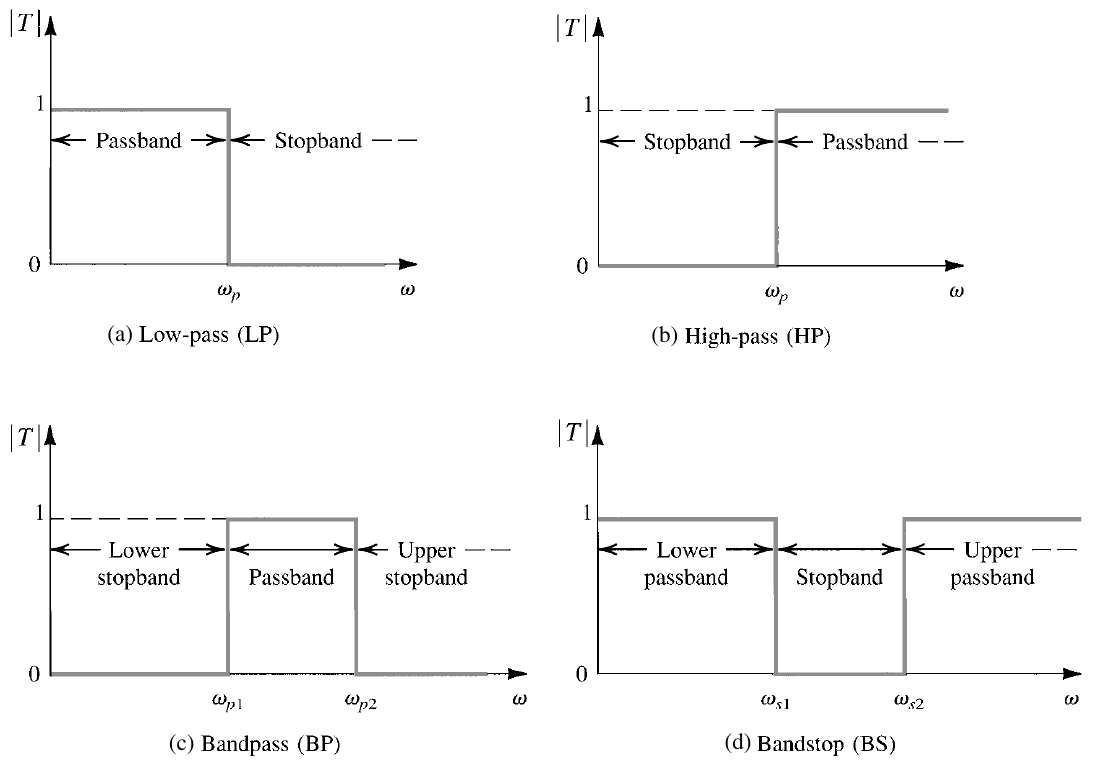
\includegraphics[width=0.75\linewidth]{figures/Filter-types}
\end{figure}

\section{Filter with source}

\begin{figure}[H]
  \centering
  \begin{subfigure}{.35\textwidth}
    \centering
    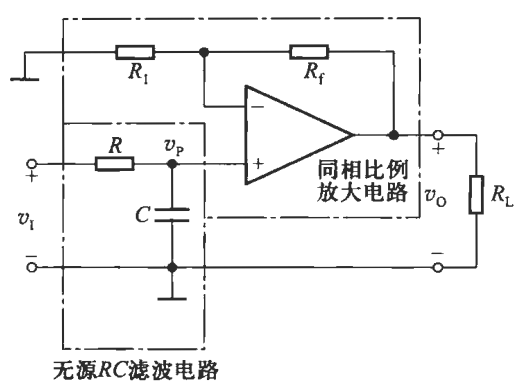
\includegraphics[width=\linewidth]{figures/Filter-with-source}
  \end{subfigure}
  \begin{subfigure}{.55\textwidth}
    \centering
    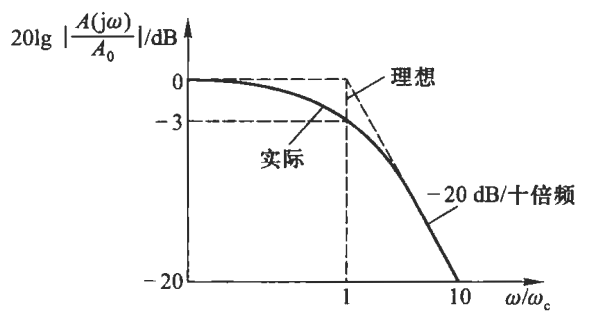
\includegraphics[width=\linewidth]{figures/Filter-with-source-graph}
  \end{subfigure}
\end{figure}

\section{Sallen-Key Filtering Circuit}

\begin{figure}[H]
  \centering
  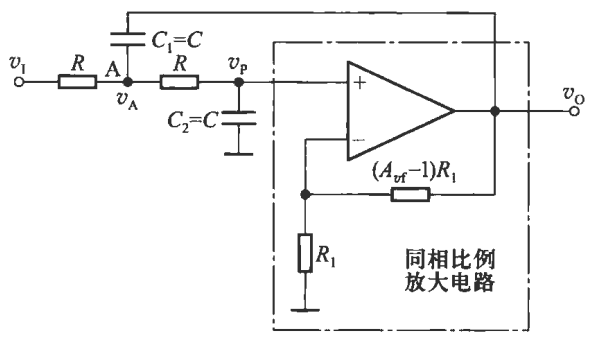
\includegraphics[width=0.5\linewidth]{figures/Sallen-Key}
\end{figure}

\section{Voltage Comparator}

\begin{figure}[H]
  \centering
  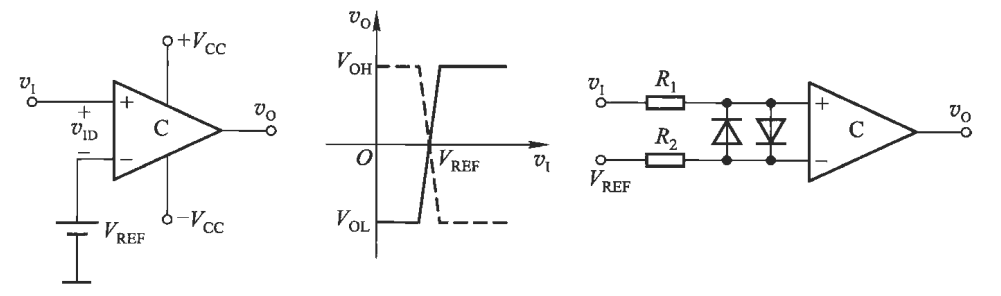
\includegraphics[width=\linewidth]{figures/Voltage-Comparator}
\end{figure}

\section{Inverting Schmitt Trigger}

\begin{figure}[H]
  \centering
  \begin{subfigure}{.45\textwidth}
    \centering
    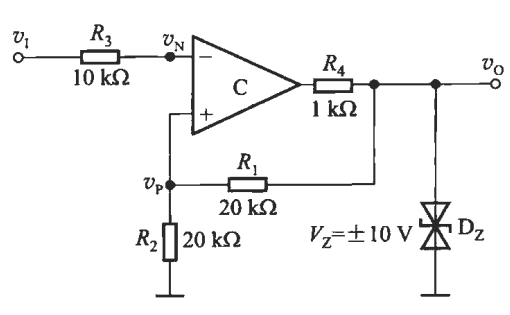
\includegraphics[width=\linewidth]{figures/Trigger-1}
  \end{subfigure}
  \quad\quad\quad\quad
  \begin{subfigure}{.35\textwidth}
    \centering
    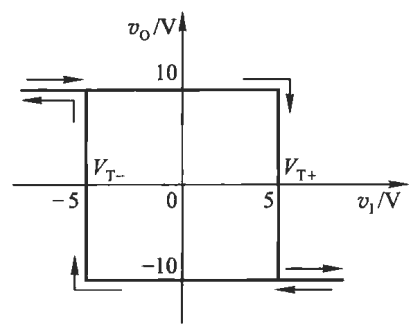
\includegraphics[width=\linewidth]{figures/Trigger-2}
  \end{subfigure}
\end{figure}

\section{RC Phase Shifting Network}

There are 3 this kind of network below, each may generate up to $90^{\circ}$ phase shift.

\begin{figure}[H]
  \centering
  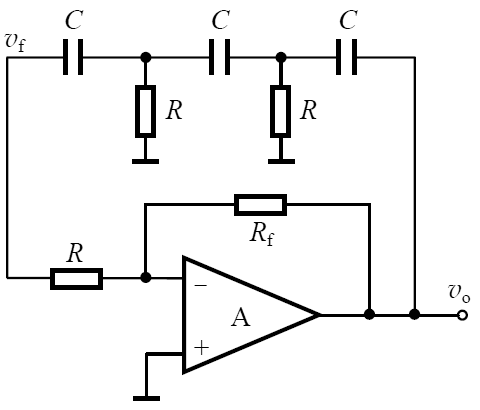
\includegraphics[width=0.5\linewidth]{figures/RC-Phase-Shifting}
\end{figure}

\section{Stability of RC Oscillator}

\begin{figure}[H]
  \centering
  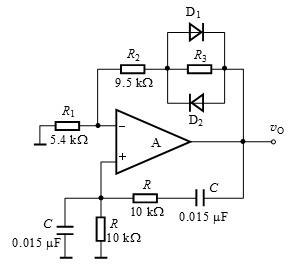
\includegraphics[width=0.5\linewidth]{figures/Stability-RC-Oscillator}
\end{figure}

\begin{equation*}
  \begin{aligned}
    A_V = 1 + \dfrac{R_2 + \left( R_3 \parallel R_D \right)}{R_1} > 3 
  \end{aligned}
\end{equation*}

\section{RC Phase Selecting Network}

\begin{figure}[H]
  \centering
  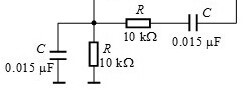
\includegraphics[width=0.5\linewidth]{figures/RC-Selecting-Network}
\end{figure}

\begin{equation*}
  \begin{aligned}
    f = \dfrac{1}{2 \pi RC}  
  \end{aligned}
\end{equation*}



\section{Generation of Square Waveforms}

\begin{figure}[H]
  \centering
  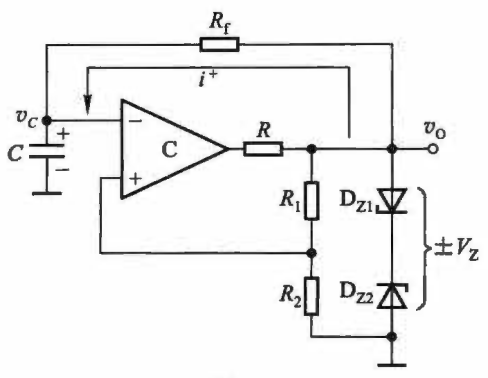
\includegraphics[width=0.5\linewidth]{figures/Square}
\end{figure}

\section{Generation of Triangle Waveforms}

\begin{figure}[H]
  \centering
  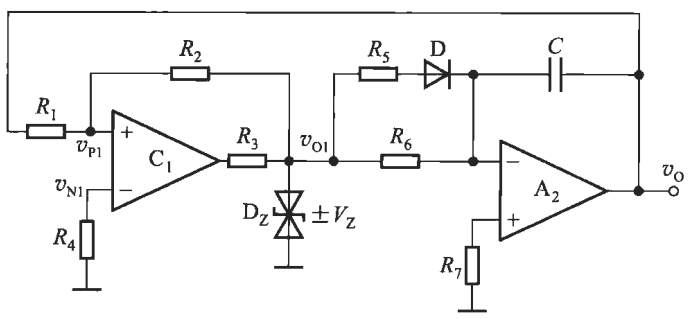
\includegraphics[width=0.8\linewidth]{figures/Triangle}
\end{figure}

%%% Local Variables:
%%% mode: latex
%%% TeX-master: "Analogue_Electronics"
%%% End:
